\documentclass[a4paper,11pt]{article}
\usepackage{ctex}
\usepackage{enumerate}
\usepackage{times}
\usepackage{mathptmx}
\usepackage{amsmath}
\usepackage{amssymb}
\usepackage{tikz}
\usepackage[top=2cm, bottom=2cm, left=2cm, right=2cm]{geometry}

\allowdisplaybreaks[4]
\renewcommand{\labelenumi}{(\alph{enumi})}
\newcommand{\set}[1]{\{#1\}}
\newcommand{\diam}{\mathop{\mathrm{diam}}}
\begin{document}
  \title{����~2-15~��ҵ}
  \author{��������ۿԴ \and ѧ�ţ�161240004}
  \date{}
  \maketitle

  \section{[CZ] Problem 1.6}
  $F = (V, E)$ \par
  $V = \set{c_1, c_2, \cdots, c_{12}}$ \par
  $E = \set{\set{c_1, c_5}, \set{c_1, c_6}, \set{c_1, c_8}, \set{c_1, c_9}, \set{c_2, c_7}, \set{c_2, c_{10}}, \set{c_3, c_7}, \set{c_3, c_{10}}, \set{c_4, c_8}, \set{c_4, c_9}, \set{c_4, c_{10}}, \\ \set{c_4, c_{11}}, \set{c_4, c_{12}}, \set{c_5, c_{10}}, \set{c_6, c_{10}}, \set{c_7, c_{11}}, \set{c_7, c_{12}}}$

  \section{[CZ] Problem 1.8}
  \begin{enumerate}
    \item The words in $S_1$ are (presented from left to right): cat, cap, tap, top. \par
    The words in $S_2$ are: map (center) , mop, tap, mat (surrounding). \par
    The words in $S_3$ are: run (top left), gun (top right), sun (center), son (bottom). \par
    The words in $S_4$ are (presented clockwise): slit, slot, slop, slip. \par
    The words in $S_5$ are (presented clockwise from top left): pot, put, pet, poet. \par
    The words in $S_6$ are (presented clockwise): lake, sake, take, make.
    \item  The graph $H$ is: \par
      \begin{centering}
      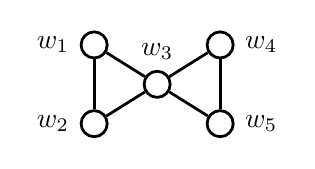
\begin{tikzpicture}[line width = 1pt,
                        solid/.style = {circle, draw, fill = black, minimum size = 0.1cm},
                        empty/.style = {circle, draw, fill = white, minimum size = 0.1cm}]
      \node [empty, label=left:$w_1$] (T1) at (0, 1){};
      \node [empty, label=left:$w_2$] (T2) at (0, 0){};
      \node [empty, label=above:$w_3$] (T3) at (0.8, 0.5){};
      \node [empty, label=right:$w_4$] (T4) at (1.6, 1){};
      \node [empty, label=right:$w_5$] (T5) at (1.6, 0){};

      \draw (T1) -- (T2);
      \draw (T4) -- (T5);
      \draw (T1) -- (T3) -- (T4);
      \draw (T2) -- (T3) -- (T5);
      \end{tikzpicture} \par
      \end{centering}
      \normalsize
      It is a word graph of some set, and the corresponding words are: top, tap, tip, lip, dip.
  \end{enumerate}
  
  \section{[CZ] Problem 1.10}
  $F = (V, E)$ \par
  $V = \set{L1, L2, \cdots, L7}$ \par
  $E = \set{\set{L1, L3}, \set{L1, L4}, \set{L1, L5}, \set{L1, L6}, \set{L2, L3}, \set{L2, L4}, \set{L4, L5}, \set{L4, L6}, \set{L5, L6}}$
  
  \section{[CZ] Problem 1.14}
  Let $C$ denote a component of $G$. \par
  (1) $\rightarrow$ (2): Take any vertex $v_0$ in $C$. For any vertex $v_i$ which is connected to $v_0$, it must in $V(C)$, otherwise if we add $v_i$, along with the edges in the path from $v_0$ to $v_i$, to $C$, we get a proper connected supergraph of $C$, which leads to contradiction. Therefore, $V(C)$ is an equivalent class. Then we have to prove $C$ is the subgraph induced by $V(C)$. If not, let $C'$ be the subgraph induced by $V(C)$, and $E(C) \subset E(C')$, thus $C$ is a proper subgraph of $C'$, which leads to contradiction.  \par
  (2) $\rightarrow$ (1): Suppose, to the contrary that $C$ is a proper subgraph of a connected subgraph of $G$, denoted by $C'$. If $V(C) \subset V(C')$, there exists some vertex connected to $C$ but not in the equivalent class, which leads to contradiction. It is impossible that $V(C) = V(C')$, because the subgraph induced by $V(C)$ is the maximal subgraph whose vertex set is $V(C)$.
  
  \section{[CZ] Problem 1.16}
  For every $i$, we have a path from $u$ to $v_i$: $(u = v_0, v_1, \cdots, v_i)$, whose length is $i$. Thus $d(u, v_i) \leq i$. \par
  Suppose, to the contrary that $d(u, v_i) < i$, i.e. there exists path $(u_0 = v_0, u_1, \cdots, u_j = v_i)$, where $j < i$. Consider the walk $(u = u_0 = v_0, u_1, \cdots, u_j = v_i, v_{i+1}, \cdots, v_k = v)$, it's a $u-v$ walk shorter than the geodesic, which leads to contradiction. \par
  Therefore, $d(u, v_i) = i$ for each integer $i$ with $1 \leq i \leq k$.
  
  \section{[CZ] Problem 1.17}
  \begin{enumerate}
    \item Assume that $P$ is an $x - z$ path and $Q$ is a $u - w$ path, where $x \neq u, v$ and $y \neq u, v$, and they do not have common vertex. Let $y$ be a vertex in $P$ and $v$ be a vertex in $Q$, then there exists a $y-v$ path $(p_0 = y, p_1, p_2, \cdots, p_n = v)$. If there exists $p_i$ such that $p_i$ ($0 < i < n$) is in $P$ or $Q$, since $P \cap Q = \varnothing$, there exists a segment of the path, from any vertex in $P$ (let it be $y$), to any vertex in $Q$ (let it be $v$), such that the vertices in the segment are not in $P$ or $Q$, except the first and the last one. Assume $x - y$ is longer than $y - z$, and $u - v$ is longer than $v - w$, consider the path $x - y - v - u$, it is longer than the $x - z$ path and the $u - v$ path, which leads to contradiction.
    \item This is true. The geodesics are as well the longest paths in $G$, otherwise $\diam(G) > k$. Apply the conclusion we've proved in (1), we obtain that $P$ and $Q$ must have at least one common vertex.
  \end{enumerate}
  
  \section{[CZ] Problem 1.18}
  \begin{enumerate}
    \item The minimum size of such a subgraph contains only the vertices and edges in a $u-v$ geodesic. Any connected subgraph containing $u$ and $v$ must have a $u-v$ path, which is at least as long as the geodesic. So a subgraph contains only the vertices and edges in a $u-v$ geodesic has less edges or vertices than other graphs.
    \item What is the maximum size of a connected subgraph of $G$ containing $u$ and $v$? It is $G$.
  \end{enumerate}
\end{document}
